\documentclass[usenames,dvipsnames, 18pt, compress, aspectratio=169]{beamer}

% can be compiled by xelatex -shell-escape presentation.tex
% lualatex -shell-escape presentation.tex

\usetheme[]{metropolis}

\usepackage[utf8]{inputenc}
\usepackage[russian, english]{babel}
\usepackage{booktabs}
\usepackage[scale=2]{ccicons}
\usepackage{listings}
\usepackage{marvosym}
\usepackage{color}
\usepackage{xcolor}
\usepackage[document]{ragged2e}
\usepackage[export]{adjustbox}
\usepackage{fontawesome5}
\usepackage{enumitem}
\usepackage{minted}
\usemintedstyle{tango}
\usepackage[normalem]{ulem}
\usepackage{amsmath}
\usepackage{amsthm}
\usepackage{amssymb}
\usepackage{mathtools, nccmath}
\usepackage{wrapfig}
\usepackage{comment}
\usepackage{tikz}
\usetikzlibrary{patterns}
\usetikzlibrary{mindmap}
\usetikzlibrary{shapes.misc, fit}
\usetikzlibrary{spy, decorations, decorations.pathmorphing, decorations.pathreplacing, backgrounds, decorations.text}
\usepackage{graphicx}
\usepackage{xspace}
\usepackage{eso-pic}
\usepackage{verbatim}
\usepackage{smartdiagram}
\usesmartdiagramlibrary{additions}
\usetikzlibrary{trees}
\usepackage{datetime}
\usepackage{hyperref}
\usepackage{forloop}
\usepackage{copyrightbox}
\usepackage{csquotes}
\usepackage{hyperref}
\usepackage{pgfplots}
\usetikzlibrary{tikzmark}
\usetikzlibrary{arrows.meta}

\usepackage{tcolorbox}
\usepackage{tabularx}
\usepackage{array}
\usepackage{colortbl}
\tcbuselibrary{skins}

\usetikzlibrary{shapes,arrows,positioning}
\graphicspath{{images/}}

\def\social{{\faMastodon}}
\def\github{{\faGithub}}
\def\email{{\faEnvelope}}
\def\search{{\faSearch}}

\renewcommand{\ttdefault}{pcr}
\setmonofont{FiraCode-VF}

\usefonttheme{professionalfonts} % using non standard fonts for beamer
\usefonttheme{serif} % default family is serif
\usepackage{fontspec}
\setmainfont{Liberation Sans}
\newfontfamily\ExtraLight{Liberation Sans}
\newfontfamily\Light{Liberation Sans}
\newfontfamily\Book{Liberation Sans}
\newfontfamily\Medium{Liberation Sans}

\makeatletter
\newcommand\HUGE{\@setfontsize\Huge{32}{41}}
\makeatother

\newcommand\AtPagemyUpperLeft[1]{\AtPageLowerLeft{%
\put(\LenToUnit{0.85\paperwidth},\LenToUnit{0.05\paperheight}){#1}}}

\newcommand\AtPagemyUpperTop[1]{\AtPageLowerLeft{%
\put(\LenToUnit{0.42\paperwidth},\LenToUnit{0.90\paperheight}){#1}}}

\renewcommand{\ULthickness}{2.0pt}

\newcommand{\highlight}[2]{\colorbox{#1!17}{$\displaystyle #2$}}
\renewcommand{\highlight}[2]{\colorbox{#1!17}{#2}}

\definecolor{links}{HTML}{0099FF}
\hypersetup{colorlinks, linkcolor=, urlcolor=links}
\definecolor{greenGood}{HTML}{99FF99}
\definecolor{redBad}{HTML}{FF9980}
\definecolor{title}{HTML}{ee0000}
\definecolor{subtitle}{HTML}{ee0000}

\setbeamerfont{section title}{family=\Book, size=\Huge, shape=\normalfont}
\setbeamerfont{frametitle}{family=\Book, size=\large, shape=\normalfont}
\setbeamerfont{title}{family=\Book, size=\Large, shape=\normalfont}
\setbeamerfont{subtitle}{size=\small}
\setbeamerfont{author}{family=\ExtraLight, size=\footnotesize}

\definecolor{cec1d24}{RGB}{236,29,36}
\definecolor{cffffff}{RGB}{255,255,255}
\tikzset{>=latex}

\setbeamertemplate{navigation symbols}{}
\beamertemplatenavigationsymbolsempty
\pagenumbering{gobble}

\SetBlockThreshold{0}

\tcbset{
    on line,
    boxsep=4pt,
    left=0pt,
    right=0pt,
    top=0pt,
    bottom=0pt,
    colframe=white
}

\tikzset{btree-line/.style={line width=0.5pt}}

\tikzset{btree-node/.style={
    draw,
    inner sep=0,
    minimum width=1cm,
    minimum height=1cm,
    rounded corners
}}

\tikzset{btree-leaf-node/.style={btree-node, fill=greenGood}}
\tikzset{btree-branch-node/.style={btree-node, fill=gray!20}}

\newcommand{\basicbtree}[2] {
    \node[btree-branch-node] (node1) {};

    \node[btree-branch-node, below=0.5cm of node1.south west, xshift=-2.5cm] (node2) {};
    \node[btree-branch-node, below=0.5cm of node1.south] (node3) {};
    \node[btree-branch-node, below=0.5cm of node1.south east, xshift=2.5cm] (node4) {};

    \node[btree-leaf-node, below=0.5cm of node2.south west, xshift=-0.2cm] (node5) {};
    \node[btree-leaf-node, below=0.5cm of node2.south east, xshift=0.2cm] (node6) {};

    \node[btree-leaf-node, below=0.5cm of node3.south west, xshift=-0.2cm] (node7) {};
    \node[btree-leaf-node, below=0.5cm of node3.south east, xshift=0.2cm] (node8) {};

    \node[btree-leaf-node, below=0.5cm of node4.south west, xshift=-0.2cm] (node9) {};
    \node[btree-leaf-node, below=0.5cm of node4.south east, xshift=0.2cm] (node10) {#2};

    \ifthenelse{ \equal{#1}{show-connections} } {
        \draw[->, btree-line] (node1) -- (node2);
        \draw[->, btree-line] (node1) -- (node3);
        \draw[->, btree-line] (node1) -- (node4);

        \draw[->, btree-line] (node2) -- (node5);
        \draw[->, btree-line] (node2) -- (node6);

        \draw[->, btree-line] (node3) -- (node7);
        \draw[->, btree-line] (node3) -- (node8);

        \draw[->, btree-line] (node4) -- (node9);
        \draw[->, btree-line] (node4) -- (node10);
    } {}

    \ifthenelse{ \equal{#1}{show-fade-connections} } {
        \draw[->, btree-line, color=gray] (node1) -- (node2);
        \draw[->, btree-line, color=gray] (node1) -- (node3);
        \draw[->, btree-line, color=gray] (node1) -- (node4);

        \draw[->, btree-line, color=gray] (node2) -- (node5);
        \draw[->, btree-line, color=gray] (node2) -- (node6);

        \draw[->, btree-line, color=gray] (node3) -- (node7);
        \draw[->, btree-line, color=gray] (node3) -- (node8);

        \draw[->, btree-line, color=gray] (node4) -- (node9);
        \draw[->, btree-line, color=gray] (node4) -- (node10);
    } {}
}


\setbeamertemplate{title page}
{

  \vspace*{2.1cm}
  \hspace{5.5cm}
  \begin{minipage}[b][\paperheight]{0.7\textwidth}
  \begin{center}

    \ifx\inserttitle\@empty\else
    {{% \inserttitle is nonempty
      \raggedright%
      %\linespread{1.0}%
      \usebeamerfont{title}%
      \usebeamercolor[fg]{title}%
      %\vspace*{1.3em}
      \if@noSmallCapitals%
        \inserttitle%
      \else%
        \scshape{\color{title} \textbf{\begin{flushleft}\inserttitle\end{flushleft}}}%
      \fi%
      \vspace*{0.3em}
    }}
    \fi

    %\vspace*{0.5em}%

    \ifx\insertsubtitle\@empty\else
    {{% \insertsubtitle is nonempty
      \usebeamerfont{subtitle}%
      \usebeamercolor[fg]{subtitle}%
      {\color{subtitle} \begin{flushleft}\insertsubtitle\end{flushleft}}%
      \vspace*{3.0em}%
    }}
    \fi

    \vspace*{1.0em}%

    \usebeamerfont{author}%
    \usebeamercolor[fg]{author}%
    {\begin{flushleft}\color{black} \insertauthor\end{flushleft}}%

    %\vspace*{1.5em}
    \fontsize{8pt}{10}\selectfont
    {\begin{flushleft}\color{black} 14-03-2024\end{flushleft}}%

    \vfill
    \vspace*{2em}
  \end{center}
  \end{minipage}
}

\setbeamertemplate{section page}
{
  \vspace{2em}
  \centering
  \begin{minipage}{22em}
    \usebeamercolor[fg]{section title}
    \usebeamerfont{section title}
    {\color{black} \insertsectionhead\\[-1ex]}
  \end{minipage}
  \par
}

\setbeamertemplate{footline}
{
\begin{beamercolorbox}[wd=\textwidth,ht=3ex,dp=3ex,leftskip=0.3cm,rightskip=0.3cm]{structure}
  \usebeamerfont{page number in head/foot}
  \insertframenumber
\end{beamercolorbox}
}

\pgfmathdeclarefunction{gauss}{2}{%
  \pgfmathparse{1/(#2*sqrt(2*pi))*exp(-((x-#1)^2)/(2*#2^2))}%
}

\pgfmathdeclarefunction{longtail}{2}{%
  \pgfmathparse{1/(#2*sqrt(2*pi))*exp(-(pow((ln(x)-#1),2))/(2*#2^2))}%
}

\title{Calculating the future}
\subtitle{How to model PostgreSQL performance}
\date{\today}
\author{Dmitrii Dolgov}
\institute{}

\begin{document}
{
  \usebackgroundtemplate{
\includegraphics[width=\paperwidth]{title.png}}%
  \fontsize{17pt}{18}\selectfont
  \maketitle
}

\AddToShipoutPictureBG{
  \AtPagemyUpperLeft{{
\includegraphics[width=2.0cm,keepaspectratio]{logo.png}}}
}

\fontsize{17pt}{18}\selectfont

\setbeamertemplate{background canvas}{}

\begin{frame}[fragile]{}
    \frametitle{}
    \begin{itemize}[label={\MVRightarrow }]
        \item Why is it relevant for you? % motivation
        \item Back of the envelope calculations % space and bloat
        \item Approximation % IO cost model
        \item Simulation % query latency
    \end{itemize}
\end{frame}

\section{Why bother?}

\begin{frame}[fragile]{}
    \frametitle{}
    \begin{itemize}[label={}]
        \item <+-> \textbf{Benchmarking instead?} \vspace{0.5cm}
        \item <+-> \MVRightarrow \hspace{0.1cm} Resource intensive % money and time
        \item <+-> \MVRightarrow \hspace{0.1cm} Hard to get full coverage
        \item <+-> \MVRightarrow \hspace{0.1cm} Requires cross validation \vspace{0.5cm}
        \item <+-> \textbf{Enhance benchmarking!}
    \end{itemize}
\end{frame}

\begin{frame}[fragile]{}
    \frametitle{}
    \begin{itemize}[label={}]
        \item <+-> \textbf{It's easy} \vspace{0.5cm}
        \item <+-> \MVRightarrow \hspace{0.1cm} just bump max\_wal\_size?
        \item <+-> \MVRightarrow \hspace{0.1cm} just increase shared\_buffers?
        \item <+-> \MVRightarrow \hspace{0.1cm} just configure autovacuum? \vspace{0.5cm}
        \item <+-> \textbf{Well...}
    \end{itemize}
\end{frame}

\begin{frame}[fragile]{}
    \frametitle{}

    \begin{center}
    \copyrightbox[b]
    {
        \includegraphics
        [width=1.1\textwidth,center]
        {bridge.png}
    }
    {
        Douglas A. Nettleton, John S. Torkelson Department of Transportation,
        Federal Highway Administration, Office of Engineering, Bridge Division
    }

    \end{center}
\end{frame}
\note{
    https://en.wikipedia.org/wiki/File:Arch_bridge_nomenclature.png

    It's obvious that the pillars have to be large, but how large/thick? What
    are the maintenance costs, what is the stress long term due to weather and
    other changes?
}

\begin{frame}[fragile]{}
    \frametitle{}

    \begin{center}
    \copyrightbox[b]
    {
        \includegraphics
        [width=0.9\textwidth,center]
        {map.png}
    } { \hspace{5.0cm} OSM }

    \end{center}
\end{frame}
\note{
    Going one level higher, how the bridge will affect the environment,
    traffic, etc?

    In the end the goal is to start doing database engineering by the standards
    of civil engineering.
}

\section{Target of the experiment}

\begin{frame}[fragile]{}
    \frametitle{}

    \begin{overprint}[\textwidth]
        \onslide<1>
        \begin{minted}[fontsize=\Large,escapeinside=||]{sql}
        create table test(a int);
        create index on |\colorbox{white}{\textbf{test(a)}}|;
        \end{minted}

        \onslide<2>
        \begin{minted}[fontsize=\Large,escapeinside=||]{sql}
        create table test(a int);
        create index on |\colorbox{RedOrange}{\textbf{test(a)}}|;
        \end{minted}
    \end{overprint}

\end{frame}

\section{Back of the envelope\\ calculations}

%\begin{frame}[fragile]{}
    %\frametitle{}

    %\blockquote{\it
        %[...] we present a minimal, parsimonious model to account for the cost
        %of maintaining a high body temperature [...]. A body temperature of
        %36.7°C maximizes fitness by restricting the growth of most fungal
        %species relative to its metabolic cost.
    %}

    %\linespread{0.5}
    %\vspace{0.5cm}
    %\color{black}\fontsize{6pt}{0}\selectfont
        %Bergman A, Casadevall A. 2010. Mammalian Endothermy Optimally Restricts
        %Fungi and Metabolic Costs. mBio 1:10.1128/mbio.00212-10.
        %https://doi.org/10.1128/mbio.00212-10
    %\linespread{1.5}

%\end{frame}
%\note{
    %https://journals.asm.org/doi/full/10.1128/mbio.00212-10
%}

\begin{frame}[fragile]{}
    \frametitle{}

    Assuming we know the schema,\\
    how to approximate space usage?
\end{frame}

\begin{frame}[fragile]{}
    \frametitle{}

    \begin{overprint}[\textwidth]
        \onslide<1>
        \begin{minted}[fontsize=\Large,escapeinside=||]{sql}
        create table test(a int);
        create index on test(a);
        \end{minted}

        \onslide<2>
        \begin{minted}[fontsize=\Large,escapeinside=||]{sql}
        create table test(a int);
        create index on test(a)
            with (fillfactor = 100);
        \end{minted}
    \end{overprint}

\end{frame}

\begin{frame}[fragile]{}
    \frametitle{}

    \begin{center}
        \begin{overprint}[14cm]
        \onslide<1>
        \begin{tikzpicture}[]
            \basicbtree{show-connections}{}
            \draw[decoration={brace,mirror,raise=5pt,amplitude=5pt},decorate,line width=1.5pt,color=white]
                  ([xshift=-0.5cm]node5.north west) -- node[left=7pt,color=white] {~99\%} ([xshift=-0.5cm]node5.south west);
        \end{tikzpicture}

        \onslide<2>
        \begin{tikzpicture}[]
            \basicbtree{show-connections}{}
            \draw[decoration={brace,mirror,raise=5pt,amplitude=5pt},decorate,line width=1.5pt]
                  ([xshift=-0.5cm]node5.north west) -- node[left=7pt] {~99\%} ([xshift=-0.5cm]node5.south west);
        \end{tikzpicture}

        \linespread{0.5}
        \vspace{0.5cm} \hspace{2.0cm}
        \color{black}\fontsize{6pt}{0}\selectfont
            Goetz Graefe. "Modern B-Tree Techniques." Foundations and Trends in
            Databases 3.4 (2010) 203-402
        \linespread{1.5}

        \onslide<3>
        \begin{tikzpicture}[]
            \basicbtree{show-connections}{\search}
            \draw[decoration={brace,mirror,raise=5pt,amplitude=5pt},decorate,line width=1.5pt]
                  ([xshift=-0.5cm]node5.north west) -- node[left=7pt] {~99\%} ([xshift=-0.5cm]node5.south west);
        \end{tikzpicture}

        \linespread{0.5}
        \vspace{0.5cm} \hspace{2.0cm}
        \color{black}\fontsize{6pt}{0}\selectfont
            Goetz Graefe. "Modern B-Tree Techniques." Foundations and Trends in
            Databases 3.4 (2010) 203-402
        \linespread{1.5}

        \end{overprint}
    \end{center}

\end{frame}

\begin{frame}[fragile]{}
    \frametitle{}

    \begin{overprint}[8cm]
    \onslide<1>
    \begin{tikzpicture}[]
        \node[] at (2,1) {8192 / 0000};
        \draw[
            line width=0.5mm,
            rounded corners=0.2cm,
        ] (0,0) rectangle (14,-5) node[pos=.5] {};
    \end{tikzpicture}

    \onslide<2>
    \begin{tikzpicture}[]
        \node[] at (2,1) {8192 / 0040};
        \draw[
            line width=0.5mm,
            rounded corners=0.2cm,
        ] (0,0) rectangle (14,-5) node[pos=.5] {};

        % page header
        \draw[
            line width=0.5mm,
            rounded corners=0.2cm,
            fill=blue!17,
        ] (0.1,-0.1) rectangle (2,-1) node[pos=.5] {24};

        % index am
        \draw[
            line width=0.5mm,
            rounded corners=0.2cm,
            fill=blue!17,
        ] (12.5,-4.1) rectangle (13.9,-4.9) node[pos=.5] {16};
    \end{tikzpicture}

    \onslide<3>
    \begin{tikzpicture}[]
        \node[] at (2,1) {8192 / 1668};
        \draw[
            line width=0.5mm,
            rounded corners=0.2cm,
        ] (0,0) rectangle (14,-5) node[pos=.5] {};

        % page header
        \draw[
            line width=0.5mm,
            rounded corners=0.2cm,
            fill=blue!17,
        ] (0.1,-0.1) rectangle (2,-1) node[pos=.5] {24};

        % index am
        \draw[
            line width=0.5mm,
            rounded corners=0.2cm,
            fill=blue!17,
        ] (12.5,-4.1) rectangle (13.9,-4.9) node[pos=.5] {16};

        % item pointers
        \draw[
            line width=0.5mm,
            rounded corners=0.2cm,
            fill=green!17,
        ] (2.1,-0.1) rectangle (13.9,-1) node[pos=.5] {4 $\times$ 407};

        \draw[
            line width=0.5mm,
            rounded corners=0.2cm,
            fill=green!17,
        ] (0.1,-1.1) rectangle (6.9,-2) node[pos=.5] {};

        \draw[
            line width=0.5mm,
            rounded corners=0.2cm,
            fill=green!17,
        ] (2.1,-0.1) rectangle (3.5,-1) node[pos=.5] {4};

        \draw[
            line width=0.5mm,
            rounded corners=0.2cm,
            fill=green!17,
        ] (3.5,-0.1) rectangle (5.0,-1) node[pos=.5] {4};

        \draw[
            line width=0.5mm,
            rounded corners=0.2cm,
            fill=green!17,
        ] (5.0,-0.1) rectangle (6.5,-1) node[pos=.5] {$\cdots$};
    \end{tikzpicture}

    \onslide<4>
    \begin{tikzpicture}[]
        \node[] at (2,1) {8192 / 8180};
        \draw[
            line width=0.5mm,
            rounded corners=0.2cm,
        ] (0,0) rectangle (14,-5) node[pos=.5] {};

        % page header
        \draw[
            line width=0.5mm,
            rounded corners=0.2cm,
            fill=blue!17,
        ] (0.1,-0.1) rectangle (2,-1) node[pos=.5] {24};

        % index am
        \draw[
            line width=0.5mm,
            rounded corners=0.2cm,
            fill=blue!17,
        ] (12.5,-4.1) rectangle (13.9,-4.9) node[pos=.5] {16};

        % item pointers
        \draw[
            line width=0.5mm,
            rounded corners=0.2cm,
            fill=green!17,
        ] (2.1,-0.1) rectangle (13.9,-1) node[pos=.5] {4 $\times$ 407};

        \draw[
            line width=0.5mm,
            rounded corners=0.2cm,
            fill=green!17,
        ] (0.1,-1.1) rectangle (6.9,-2) node[pos=.5] {};

        \draw[
            line width=0.5mm,
            rounded corners=0.2cm,
            fill=green!17,
        ] (2.1,-0.1) rectangle (3.5,-1) node[pos=.5] {4};

        \draw[
            line width=0.5mm,
            rounded corners=0.2cm,
            fill=green!17,
        ] (3.5,-0.1) rectangle (5.0,-1) node[pos=.5] {4};

        \draw[
            line width=0.5mm,
            rounded corners=0.2cm,
            fill=green!17,
        ] (5.0,-0.1) rectangle (6.5,-1) node[pos=.5] {$\cdots$};

        % item data
        \draw[
            line width=0.5mm,
            rounded corners=0.2cm,
        ] (8.1,-1.1) rectangle (13.9,-2) node[pos=.5] {};

        \draw[
            line width=0.5mm,
            rounded corners=0.2cm,
            fill=red!17,
        ] (0.1,-2.1) rectangle (13.9,-3) node[pos=.5] {};

        \draw[
            line width=0.5mm,
            rounded corners=0.2cm,
            fill=red!17,
        ] (0.1,-3.1) rectangle (13.9,-4) node[pos=.5] {16 $\times$ 407};

        \draw[
            line width=0.5mm,
            rounded corners=0.2cm,
            fill=red!17,
        ] (0.1,-4.1) rectangle (12.4,-4.9) node[pos=.5] {};

        \draw[
            line width=0.5mm,
            rounded corners=0.2cm,
            fill=red!17,
        ] (8.1,-1.1) rectangle (9.5,-2) node[pos=.5] {12};

        \draw[
            line width=0.5mm,
            rounded corners=0.2cm,
            fill=red!17,
        ] (10.0,-1.1) rectangle (11.5,-2) node[pos=.5] {12};

        \draw[
            line width=0.5mm,
            rounded corners=0.2cm,
            fill=red!17,
        ] (12.0,-1.1) rectangle (13.5,-2) node[pos=.5] {$\cdots$};
    \end{tikzpicture}

    \end{overprint}
\end{frame}
\note{
    page header - 24 bytes

    item pointer - 4 bytes
    item header (IndexTupleData) - 8 bytes (6 for t_tid (ItemPointerData) + 2 for t_info)
    item data (int 4 bytes) - 4 bytes

    item header + item data is MAXALIGN'ed to 8 bytes -> 8 + 4 = 12 -> 16

    thus every index record take 16 bytes + 4 bytes item pointer

    there is 407 items on a page, 407 * (8 + 8 + 4) + 24 = 8164 = 8192 - 28,

    so although the page is full, 28 bytes are still not taken by data.

    index am specific data is located at 8176 (pd_special), and takes 16 bytes (8192 - 8176 = 16)

    =#  SELECT * from page_header(get_raw_page('test_bloat_small_a_idx', 1));
     lsn | checksum | flags | lower | upper | special | pagesize | version | prune_xid
    -----+----------+-------+-------+-------+---------+----------+---------+-----------
     0/0 |        0 |     0 |  1652 |  1664 |    8176 |     8192 |       4 |         0
    (1 row)

    then there is a space between lower part (with header and item pointers) and
    lower part (with index items):

    1664 - 1652 = 12

    16 (index am) + 12 (space between lower and upper) = 28, amounts exactly to not
    taken space.
}

%\begin{frame}[fragile]{}
    %\frametitle{}

    %Assuming we know the workload,\\
    %how to approximate free space?
%\end{frame}

%\begin{frame}[fragile]{}
    %\frametitle{}

    %\begin{minted}[fontsize=\Large,escapeinside=||]{text}
    %-- -M prepared --rate=max-rate
    %\set aid random(0, N)
    %\end{minted}

    %\begin{minted}[fontsize=\Large,escapeinside=||]{sql}
    %-- a pre-populated table
    %insert into test values(:aid);
    %\end{minted}

%\end{frame}

%\begin{frame}[fragile]{}
    %\frametitle{}
    %\begin{center}

        %\includegraphics[width=0.8\textwidth,center]{free_space_single_page.png}

    %\end{center}
%\end{frame}

%\begin{frame}[fragile]{}
    %\frametitle{}
    %\begin{center}

        %\includegraphics[width=0.8\textwidth,center]{free_space.png}

    %\end{center}
%\end{frame}

\begin{frame}[fragile]{}
    \frametitle{}

    \begin{center}
    \copyrightbox[b]
    {
        \includegraphics
        [width=0.4\textwidth,center]
        {schrei_bloat.png}
    } { \hspace{1.8cm} Edvard Munch -- The Scream (about a bloated index) }
	\end{center}

\end{frame}
\note{
	Demo
}

\begin{frame}[fragile]{}
    \frametitle{}

    Assuming we know the workload,\\
    how to approximate bloat?
\end{frame}

\begin{frame}[fragile]{}
    \frametitle{}

    \begin{minted}[fontsize=\Large,escapeinside=||]{text}
    -- -M prepared --rate=max-rate
    \set aid random(0, N)
    \set bid random(0, N)
    \end{minted}

    \begin{minted}[fontsize=\Large,escapeinside=||]{sql}
    -- a pre-populated table
    update test set a = :aid
        where a = :bid;
    \end{minted}

\end{frame}

\begin{frame}[fragile]{}
    \frametitle{}
    \begin{center}

        \includegraphics[width=0.8\textwidth,center]{bloat-single-page-update.png}

    \end{center}
\end{frame}

\begin{frame}[fragile]{}
    \frametitle{}
    \begin{center}

        \includegraphics[width=0.8\textwidth,center]{bloat-update.png}

    \end{center}
\end{frame}

\begin{frame}[fragile]{}
    \frametitle{}

    \begin{center}
    \copyrightbox[b]
    {
        \includegraphics
        [width=0.4\textwidth,center]
        {dead_tuples.jpg}
    } { \hspace{2.0cm} Portrait de l'artiste sous les traits d'un moqueur }
	\end{center}

\end{frame}
\note{
    Make sure to use index scan, disable seqscan/bitmap scan if needed
}

\section{Approximation}

\begin{frame}[fragile]{}
    \frametitle{}

    Assuming we know the workload,\\
    how to approximate amount of IO?
\end{frame}

\begin{frame}[fragile]{}
    \frametitle{}

    \begin{overprint}[\textwidth]
        \onslide<1>
        \begin{minted}[fontsize=\Large,escapeinside=||]{sql}
      create table test(a int);
      create index on test(a)
          with (fillfactor = 100);
        \end{minted}

        \onslide<2>
        \begin{minted}[fontsize=\Large,escapeinside=||]{sql}
      create unlogged table test(a int);
      create index on test(a)
          with (fillfactor = 100);
        \end{minted}

        \onslide<3>
        \begin{minted}[fontsize=\Large,escapeinside=||]{sql}
      create unlogged table test(a int);
      create index on test(a)
          with (fillfactor = 100);

      # autovacuum = off
      # *_flush_after = 0
      # etc
        \end{minted}

    \end{overprint}

\end{frame}
\note{
    checkpoint\_timeout = 1
    checkpoint\_completion\_target = 1.0
    checkpoint\_flush\_after = 0
    max\_wal\_size = 10GB
    min\_wal\_sie = 10GB
    wal\_level = minimal
    max\_wal\_senders = 0
    wal\_writer\_flush\_after = 0
}

\begin{frame}[fragile]{}
    \frametitle{}

    \begin{minted}[fontsize=\Large,escapeinside=||]{text}
    -- -M prepared --rate=max-rate
    \set aid random(0, N)
    \end{minted}

    \begin{minted}[fontsize=\Large,escapeinside=||]{sql}
    -- a pre-populated table
    select * from test where a = :aid;
    \end{minted}

\end{frame}

\begin{frame}[fragile]{}
    \frametitle{}
    \begin{center}

        \includegraphics[width=0.8\textwidth,center]{read.png}

    \end{center}
\end{frame}

\begin{frame}[fragile]{}
    \frametitle{}

    \begin{minted}[fontsize=\Large,escapeinside=||]{text}
    -- -M prepared --rate=max-rate
    \set aid random(0, N)
    \end{minted}

    \begin{minted}[fontsize=\Large,escapeinside=||]{sql}
    -- an empty table
    insert into test values(:aid);
    \end{minted}

\end{frame}

\begin{frame}[fragile]{}
    \frametitle{}
    \begin{center}

        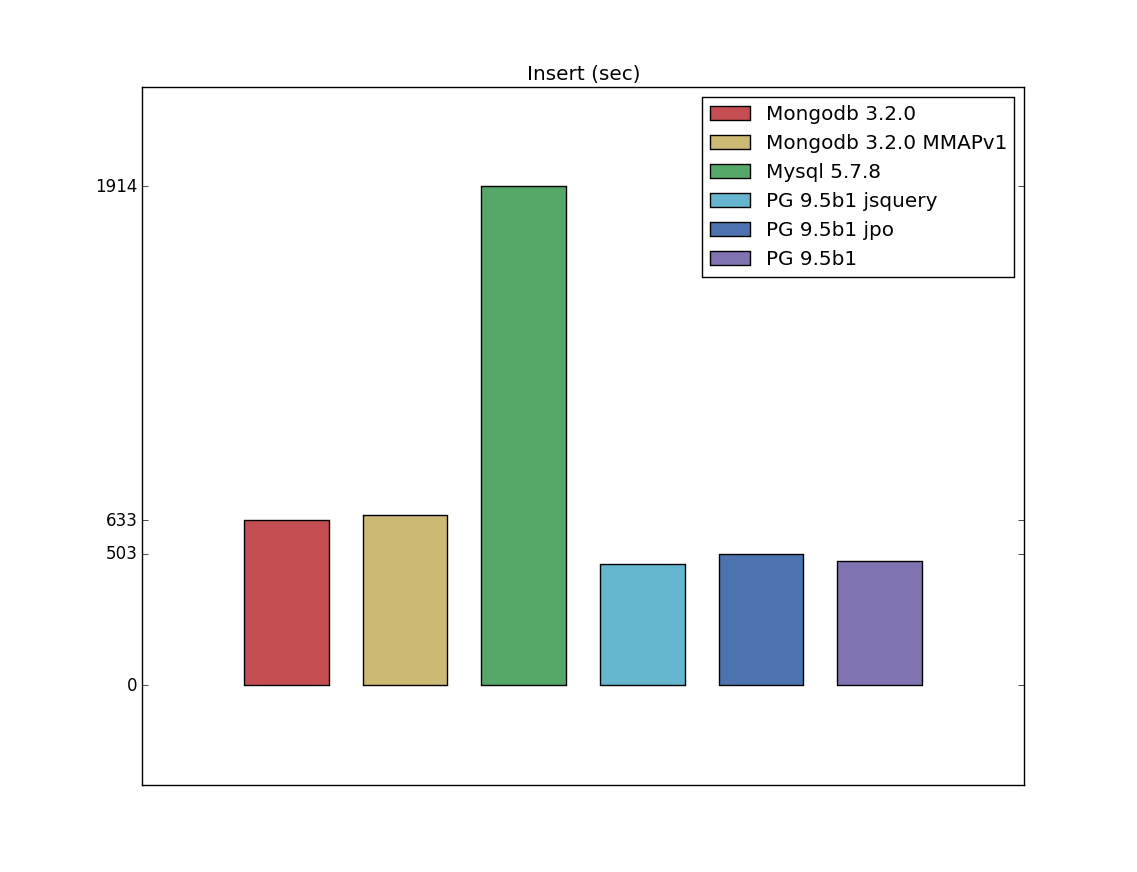
\includegraphics[width=0.8\textwidth,center]{insert.png}

    \end{center}
\end{frame}

\begin{frame}[fragile]{}
    \frametitle{}

    \begin{equation*}
        IO = \tikzmarknode{read}{\highlight{white}{$Q \cdot M_{press} \sum^{L}_{l=1}{\frac{N_l}{N}}$}} +
             \tikzmarknode{insert}{\highlight{white}{$Q_w \cdot W_g$}} +
             \tikzmarknode{split}{\highlight{white}{$\frac{Q_w}{I}$}}
    \end{equation*}\\

    \begin{tikzpicture}[overlay,remember picture,>=stealth,nodes={align=left,inner ysep=1pt},<-]
        % For "read"
        \path (read.north) ++ (0,2em) node[anchor=south east,white] (readp){Read};
        \draw [color=white](read.north) |- ([xshift=-0.3ex,color=white]readp.south west);
        % For "insert"
        \path (insert.south) ++ (-4.5em,-1.5em) node[anchor=north west,color=white] (insertp){Insert};
        \draw [color=white](insert.south) |- ([xshift=-0.3ex,color=white]insertp.south west);
        % For "split"
        \path (split.north) ++ (-0.5em,2em) node[anchor=north east,color=white] (splitp){Split};
        \draw [color=white](split.north) |- ([xshift=-0.3ex,color=white]splitp.south west);
    \end{tikzpicture}

\end{frame}

\begin{frame}[fragile]{}
    \frametitle{}

    \begin{equation*}
        IO = \tikzmarknode{read}{\highlight{red}{$Q \cdot M_{press} \sum^{L}_{l=1}{\frac{N_l}{N}}$}} +
             \tikzmarknode{insert}{\highlight{green}{$Q_w \cdot W_g$}} +
             \tikzmarknode{split}{\highlight{blue}{$\frac{Q_w}{I}$}}
    \end{equation*}\\

    \begin{tikzpicture}[overlay,remember picture,>=stealth,nodes={align=left,inner ysep=1pt},<-]
        % For "read"
        \path (read.north) ++ (0,2em) node[anchor=south east,color=red!67] (readp){Read};
        \draw [color=red!87](read.north) |- ([xshift=-0.3ex,color=red]readp.south west);
        % For "insert"
        \path (insert.south) ++ (-4.5em,-1.5em) node[anchor=north west,color=ForestGreen!67] (insertp){Insert};
        \draw [color=ForestGreen!57](insert.south) |- ([xshift=-0.3ex,color=ForestGreen]insertp.south west);
        % For "split"
        \path (split.north) ++ (-0.5em,2em) node[anchor=north east,color=blue!67] (splitp){Split};
        \draw [color=blue!57](split.north) |- ([xshift=-0.3ex,color=blue]splitp.south west);
    \end{tikzpicture}

\end{frame}
\note{
    $Q$ - total number of queries\\
    $Q_w$ - total number of write queries\\
    $M$ - buffer cache (in pages)\\
    $I$ - number of records per page\\
    $W_g(Q_w)$ - wal grouping function\\

    $L(n)$ - number of levels in the tree\\
    $N_l$ - number of pages at level l\\
    $M_{press}$ - memory pressure\\

	\begin{equation*}
		M_{press} =
			\begin{cases}
				\frac{N(t) - M}{N(t)}, N > M\\
				0, N < M
			\end{cases}
	\end{equation*}

	\begin{equation*}
		W_g(Q_w) = \frac{1} {
			(e^{a_w \cdot(w_d - 1)} + b_w) \cdot (e^{a_Q \cdot(Q_w - 1)} + b_Q)
		}
	\end{equation*}
}
\note{
    Doesn't include SLRU, mdzeroextend
}

\begin{frame}[fragile]{}
    \frametitle{}

    \begin{center}
    \includegraphics
    [width=0.7\textwidth,center]
    {modeling-fs-cache.png}

    \end{center}
\end{frame}
\note{
    The model is very limited and provides only IO "requests" via dynamic
    tracepoint, but could be combined with other models to get real IO.
}

\section{Simulation}

\begin{frame}[fragile]{}
    \frametitle{}

    Assuming we know the workload,\\
    how to approximate query latency?
\end{frame}

\begin{frame}[fragile]{}
    \frametitle{}

    \begin{minted}[fontsize=\Large]{haskell}
  data Event = PqGetByte TxLatency
             | GetCachedPlan TxLatency
             | BtGetTuple TxLatency
             | BtInsert TxLatency
             | HeapPagePrune TxLatency
             | HeapUpdate TxLatency
             | CommitTx TxLatency
             | SocketFlush TxLatency
    \end{minted}

\end{frame}

\begin{frame}[fragile]{}
    \frametitle{}
    \begin{center}

        \includegraphics[width=0.8\textwidth,center]{pq_getbyte.png}

    \end{center}
\end{frame}

\begin{frame}[fragile]{}
    \frametitle{}
    \textbf{Summary}
    \begin{itemize}[label={\MVRightarrow }]
        \item Predicting the future is possible!
        \item Be aware of limitations
        \item Reduce large system to small parts
        \item Combine with benchmarking and profiling
    \end{itemize}
\end{frame}

\fontsize{18pt}{18}\selectfont
\begin{frame}
  \vspace*{2.5cm}
  \begin{minipage}[b][\paperheight]{\textwidth}
  \begin{center}

      %\raggedright%
      \linespread{1.0}%
      \usebeamerfont{title}%
      \usebeamercolor[fg]{title}%
      \if@noSmallCapitals%
        Questions?
      \else%
        \scshape{\color{black} Questions?}%
      \fi%
      \vspace*{0.3em}

      \usebeamerfont{subtitle}%
      \fontsize{13pt}{14}\selectfont
      \usebeamercolor[fg]{subtitle}%
        \begin{itemize}[label={}]
            \item {\color{black} \social\ @erthalion@fosstodon.org}
            \item {\color{black} \email\ ddolgov at redhat dot com}
        \end{itemize}
      \vspace*{2.5em}%

    \vfill
    \vspace*{2em}
  \end{center}
  \end{minipage}

\end{frame}

\end{document}
